\renewcommand{\theequation}{\theenumi}
\begin{enumerate}[label=\arabic*.,ref=\thesubsubsection.\theenumi]
\numberwithin{equation}{enumi}
\item For a general polynomial equation of degree 2 , \\
$p(x,y) \implies Ax^2+Bxy+Cy^2+Dx+Ey+F=0$ \\
The vector form is  
\begin{align}
\vec{x}^T\myvec{A&B/2\\B/2&C}\vec{x}+\myvec{D&E}\vec{x}+F=0 \label{eq:poly}
\end{align} 

$3x^2-2\sqrt{6}x+2 = 0$  \\
The vector form from the equation is \ref{eq:poly} is 
\begin{align}
\vec{x}^T\myvec{3&0\\0&0}\vec{x}+\myvec{-2\sqrt{6}&0}\vec{x}+2 = 0
\end{align}

The values of $\vec{x}$ are found in the following python code
\begin{lstlisting}
codes/conics/example/conics.py
\end{lstlisting}

$\vec{x}=\myvec{0.81649658\\0}, \myvec{0.81649658\\0}$ \\
which can be verified from the Fig.\ref{fig:parabola}. 

The following python code generates the fig.\ref{fig:parabola}
\begin{lstlisting}
codes/conics/example/conics.py
\end{lstlisting}
\begin{figure}[!ht]
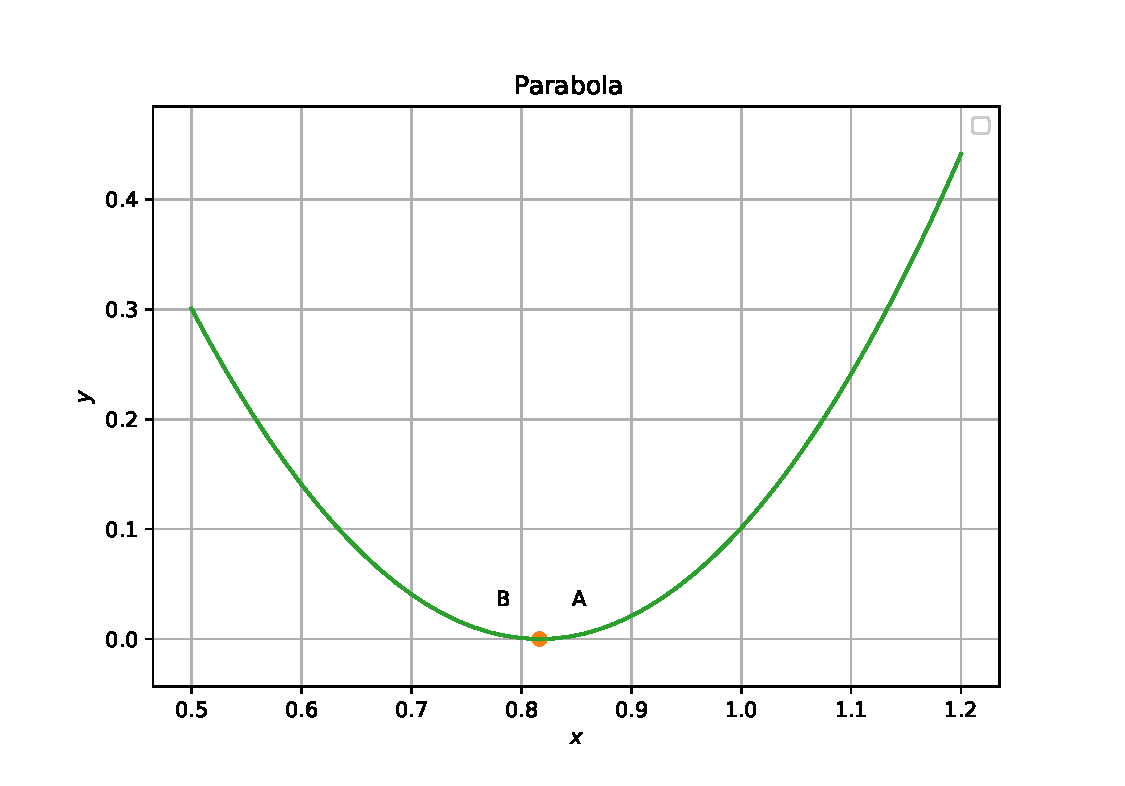
\includegraphics[width=\columnwidth]{./codes/conics/example/conics.eps}
\caption{Parabola}
\label{fig:parabola}
\end{figure} 
\end{enumerate}